\section{Compiling the Designed Circuit}


The VHDL code in the file {\it light.vhd} is processed by several 
Quartus Prime tools that analyze the code, synthesize the circuit,
and generate an implementation of it for the target chip. 
These tools are controlled by the application program called the {\it Compiler}.

Run the Compiler by selecting {\sf Processing $>$ Start Compilation}, or by 
clicking on the toolbar icon 
\includegraphics[scale=0.45]{figures/icon5.png} that looks like a
blue triangle. Your project must be saved before compiling. 
As the compilation moves through various stages, its progress is reported
in a window on the left side of the Quartus Prime display.
In the message window, at the bottom of the figure, various messages are displayed
throughout the compilation process.
In case of errors, there will be appropriate messages given.

When the compilation is finished, a compilation report is produced.
A tab showing this report is opened automatically, as seen in Figure~\ref{fig:20}.
This tab can be closed in the normal way, and it can be opened at any time
either by selecting {\sf Processing $>$ Compilation Report} or by clicking on 
the icon 
\includegraphics[scale=0.45]{figures/icon6.png}.
The report includes a number of sections listed on the left side.
Figure~\ref{fig:20} displays the Compiler Flow Summary section, which
indicates that only one logic element and three pins are needed to implement this 
tiny circuit on the selected FPGA chip.

\begin{figure}[H]
   \begin{center}
      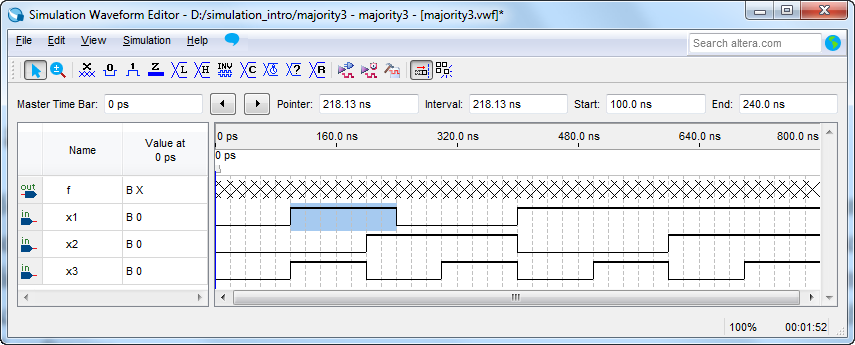
\includegraphics[scale=0.5]{figures/figure18.png}
   \caption{Display after a successful compilation.} 
	 \label{fig:18}
	 \end{center}
\end{figure}

\subsection{Errors}

The Quartus Prime software displays messages produced during compilation in the Messages window.
If the VHDL design file has been correctly specified, then one of the messages will
state that the compilation was successful and that there are no errors.

If the Compiler does not report zero errors, then there is at least one mistake 
in the VHDL code. In this case a message corresponding to each error found will
be displayed in the Messages window.  Double-clicking on an error message will highlight 
the offending statement in the VHDL code in the Text Editor window. 
Similarly, the Compiler may display some warning messages. Their details can be
explored in the same way as in the case of error messages.
The user can obtain more information about a specific error or warning message
by selecting the message and pressing the {\sf F1} function key.

To see the effect of an error, open the file {\it light.vhd}.  Remove the semicolon in the 
statement that defines the function {\it f}, illustrating a common typographical error.
Compile the erroneous design file by clicking on the 

\includegraphics[scale=.45]{figures/icon5.png} icon.
A pop-up box will ask if the changes made to the {\it light.vhd} file should be saved;
click {\sf Yes}. After trying to compile the circuit,
Quartus Prime software will display error messages in the Messages window, and 
show that the compilation failed in the {\sf Analysis \& Synthesis} stage of the compilation process.
The compilation report summary, given in Figure~\ref{fig:19}, 
confirms the failed result. In the Table of Contents panel, expand the 
{\sf Analysis \& Synthesis} part of the report
and then select {\sf Messages} to have the messages displayed as shown in Figure~\ref{fig:20}.
The Compilation Report can be displayed as a separate window as in Figure~\ref{fig:20} 
by right-clicking its tab and selecting {\sf Detach Window}, and can be reattached by clicking
{\sf Window > Attach Window}. Double-click on the first error message. 
The Quartus Prime software responds by opening the {\it light.vhd}
file and highlighting the statement which is affected by the error,
as shown in Figure~\ref{fig:21}.
Correct the error and recompile the design.

\begin{figure}[H]
   \begin{center}
      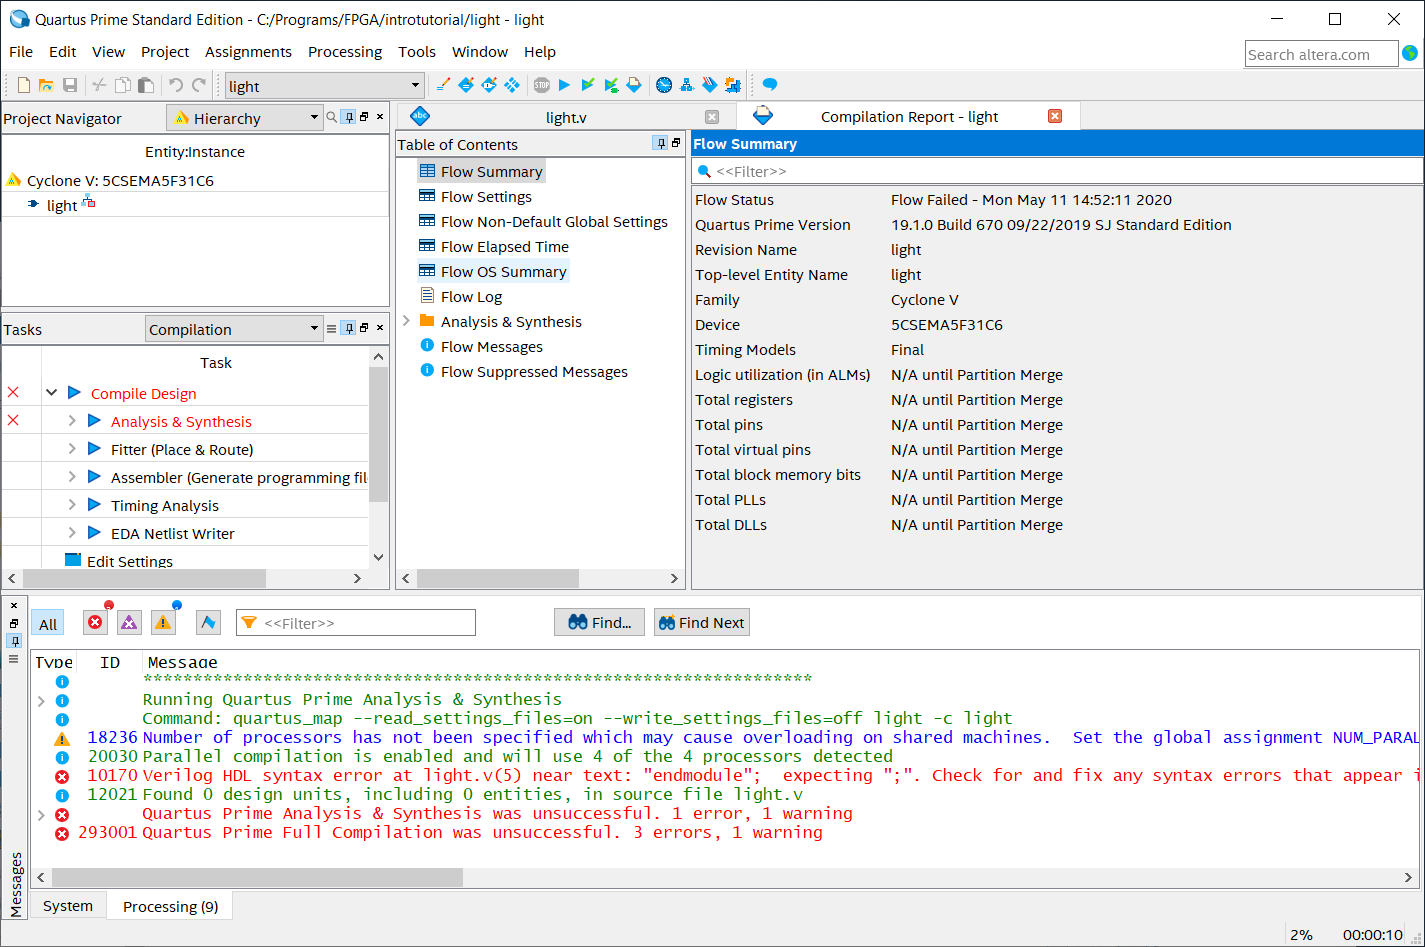
\includegraphics[scale=0.5]{figures/figure19.png}
   \caption{Compilation report for the failed design.} 
	 \label{fig:19}
	 \end{center}
\end{figure}

\begin{figure}[H]
   \begin{center}
      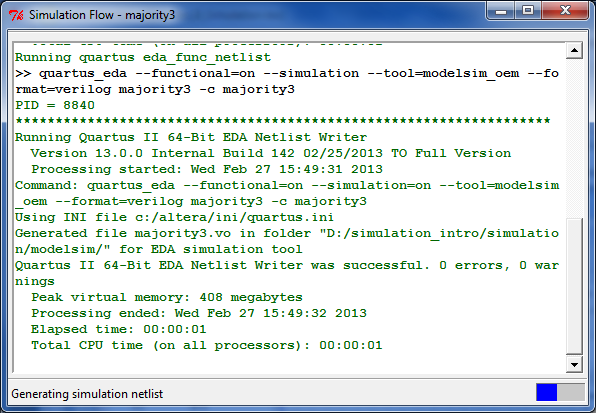
\includegraphics[scale=0.5]{figures/figure20.png}
   \caption{Error messages.}
	 \label{fig:20}
	 \end{center}
\end{figure}

\begin{figure}[H]
   \begin{center}
      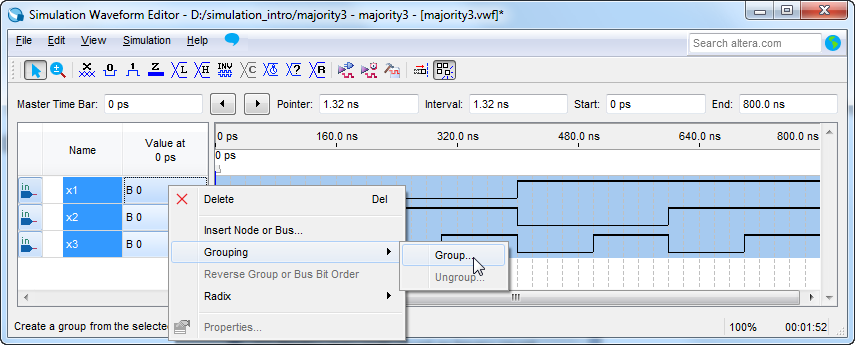
\includegraphics[scale=0.45]{figures/figure21.png}
   \caption{Identifying the location of the error.} 
	 \label{fig:21}
	 \end{center}
\end{figure}
